\documentclass[tikz,border=8pt]{standalone}
% Shared look for every TikZ diagram. Load with \input{../../tools/tikz-style.tex}
\usepackage[T1]{fontenc}
\usepackage{lmodern}
\renewcommand{\sfdefault}{lmr}  % diagrams use the same serif as the text
\usetikzlibrary{arrows.meta, positioning, shapes.geometric, calc, fit, backgrounds}
\definecolor{cblue}{HTML}{4C78A8}
\definecolor{corange}{HTML}{F58518}
\definecolor{cgreen}{HTML}{54A24B}
\definecolor{cred}{HTML}{E45756}
\definecolor{cpurple}{HTML}{B279A2}
\definecolor{cgrey}{HTML}{6B6B6B}
\tikzset{
  every picture/.style={font=\sffamily, line width=1.2pt},
  box/.style={draw=#1, fill=#1!12, rounded corners=4pt, align=center, inner sep=7pt, minimum height=1.1cm},
  box/.default=cgrey,
  arrow/.style={-{Stealth[length=3mm]}, draw=cgrey, line width=1.4pt},
  title/.style={font=\sffamily\bfseries\Large},
  note/.style={font=\sffamily\small, text=cgrey, align=center},
}
\AtBeginDocument{\hyphenpenalty=10000 \exhyphenpenalty=10000}

\begin{document}
\begin{tikzpicture}
  \begin{scope}[rotate=20]
    \draw[line width=2.2pt] (-1,0) -- (9,0) node[right] {$\pi$};
    \draw[dashed, cgrey, line width=1.4pt] (-1,1.6) -- (9,1.6) node[right, text=cgreen] {$\pi^{+}$: $w^{T}x + b = 1$};
    \draw[dashed, cgrey, line width=1.4pt] (-1,-1.6) -- (9,-1.6) node[right, text=cred] {$\pi^{-}$: $w^{T}x + b = -1$};
    \coordinate (X1) at (1.5,-1.6);
    \coordinate (X2) at (5.5,1.6);
    \node[circle, fill=cred, draw=black, inner sep=3.2pt, label={below:$x_1$}] at (X1) {};
    \node[circle, fill=cgreen, draw=black, inner sep=3.2pt, label={above:$x_2$}] at (X2) {};
    \draw[-{Stealth[length=3.5mm]}, line width=2pt, corange] (X1) -- (X2) node[midway, above left] {$x_2 - x_1$};
    \draw[-{Stealth[length=3.5mm]}, line width=2pt, cblue] (7.4,0) -- (7.4,1.0) node[right] {$\dfrac{w}{\lVert w \rVert}$};
    \draw[{Stealth[length=3mm]}-{Stealth[length=3mm]}, line width=1.4pt] (5.5,-1.6) -- (5.5,1.6);
    \draw[dotted, line width=1.2pt] (X1) -- (5.5,-1.6);
    \node[fill=white, inner sep=2pt, anchor=west] at (5.6,-0.6) {$d$};
  \end{scope}
  \node[box=cgrey, anchor=north west, text width=12.5cm, align=left] at (-0.8,-2.4)
    {$d = (x_2 - x_1)\cdot\dfrac{w}{\lVert w\rVert} = \dfrac{w^{T}x_2 - w^{T}x_1}{\lVert w\rVert} = \dfrac{(1 - b) - (-1 - b)}{\lVert w\rVert} = \dfrac{2}{\lVert w\rVert}$};
\end{tikzpicture}
\end{document}
